\subsection{Regional root-zone soil-moisture drought prediction}
\label{sec:rabi_soil}
The final software adds a distinct drought-related target: \textbf{future regional root-zone soil-water deficit}. The earlier NDVI forecast and early-drying experiment remain separate; their scores cannot be used as the accuracy of this drought model. Government declarations and satellite drying labels are not used as its training target. This is an experimental reanalysis-based risk model, not independently verified crop-loss prediction.

\subsubsection{Data, target and architecture}
Five regional cells supply 82,780 daily ERA5-Land records through April 2026, obtained through Open-Meteo. The approximate 11\,km grid does not resolve individual fields or their irrigation. Root-zone moisture is the depth-weighted mean
\[
\theta_{0:100}=0.07\theta_{0:7}+0.21\theta_{7:28}+0.72\theta_{28:100}.
\]
Seven-day means are converted to empirical percentiles using a frozen 1981--2000 reference and a calendar-day window of $\pm15$ days. A target at or below the 20th percentile is a soil-moisture deficit; at or below the 10th percentile it is severe-or-worse under this definition. Above the 20th percentile means \emph{no percentile-defined deficit}, not a healthy crop.

Issues are every five days from 1 December to 31 March. For horizon $h\in\{7,15,30\}$, the target is the seven-day mean ending at $t+h$; all seven target days are after issue. Soil and weather inputs are dated no later than $t-8$. The reference is fixed before supervised training (2001-02 to 2016-17), validation (2017-18 to 2022-23), and historical evaluation (2023-24 to 2025-26). Dates respect a simulated publication delay, but final reanalysis is not an archive of the original release vintages.

Logistic regression, random forests, histogram gradient boosting (HGB), a soil-analogue model and an equal ensemble are compared with persistence, climatology, conditional transition and damped trend. Validation average precision selects the learned model, with Brier score as a tie-breaker. Warning thresholds maximize validation $F_{0.5}$ subject to at least 50\,\% validation recall; evaluation recall is not constrained. The main selections are soil-only HGB with 7 maximum leaves at 7/15 days and 15 leaves at 30 days. These scores are not asserted to be calibrated probabilities.
\begin{figure}[H]\centering
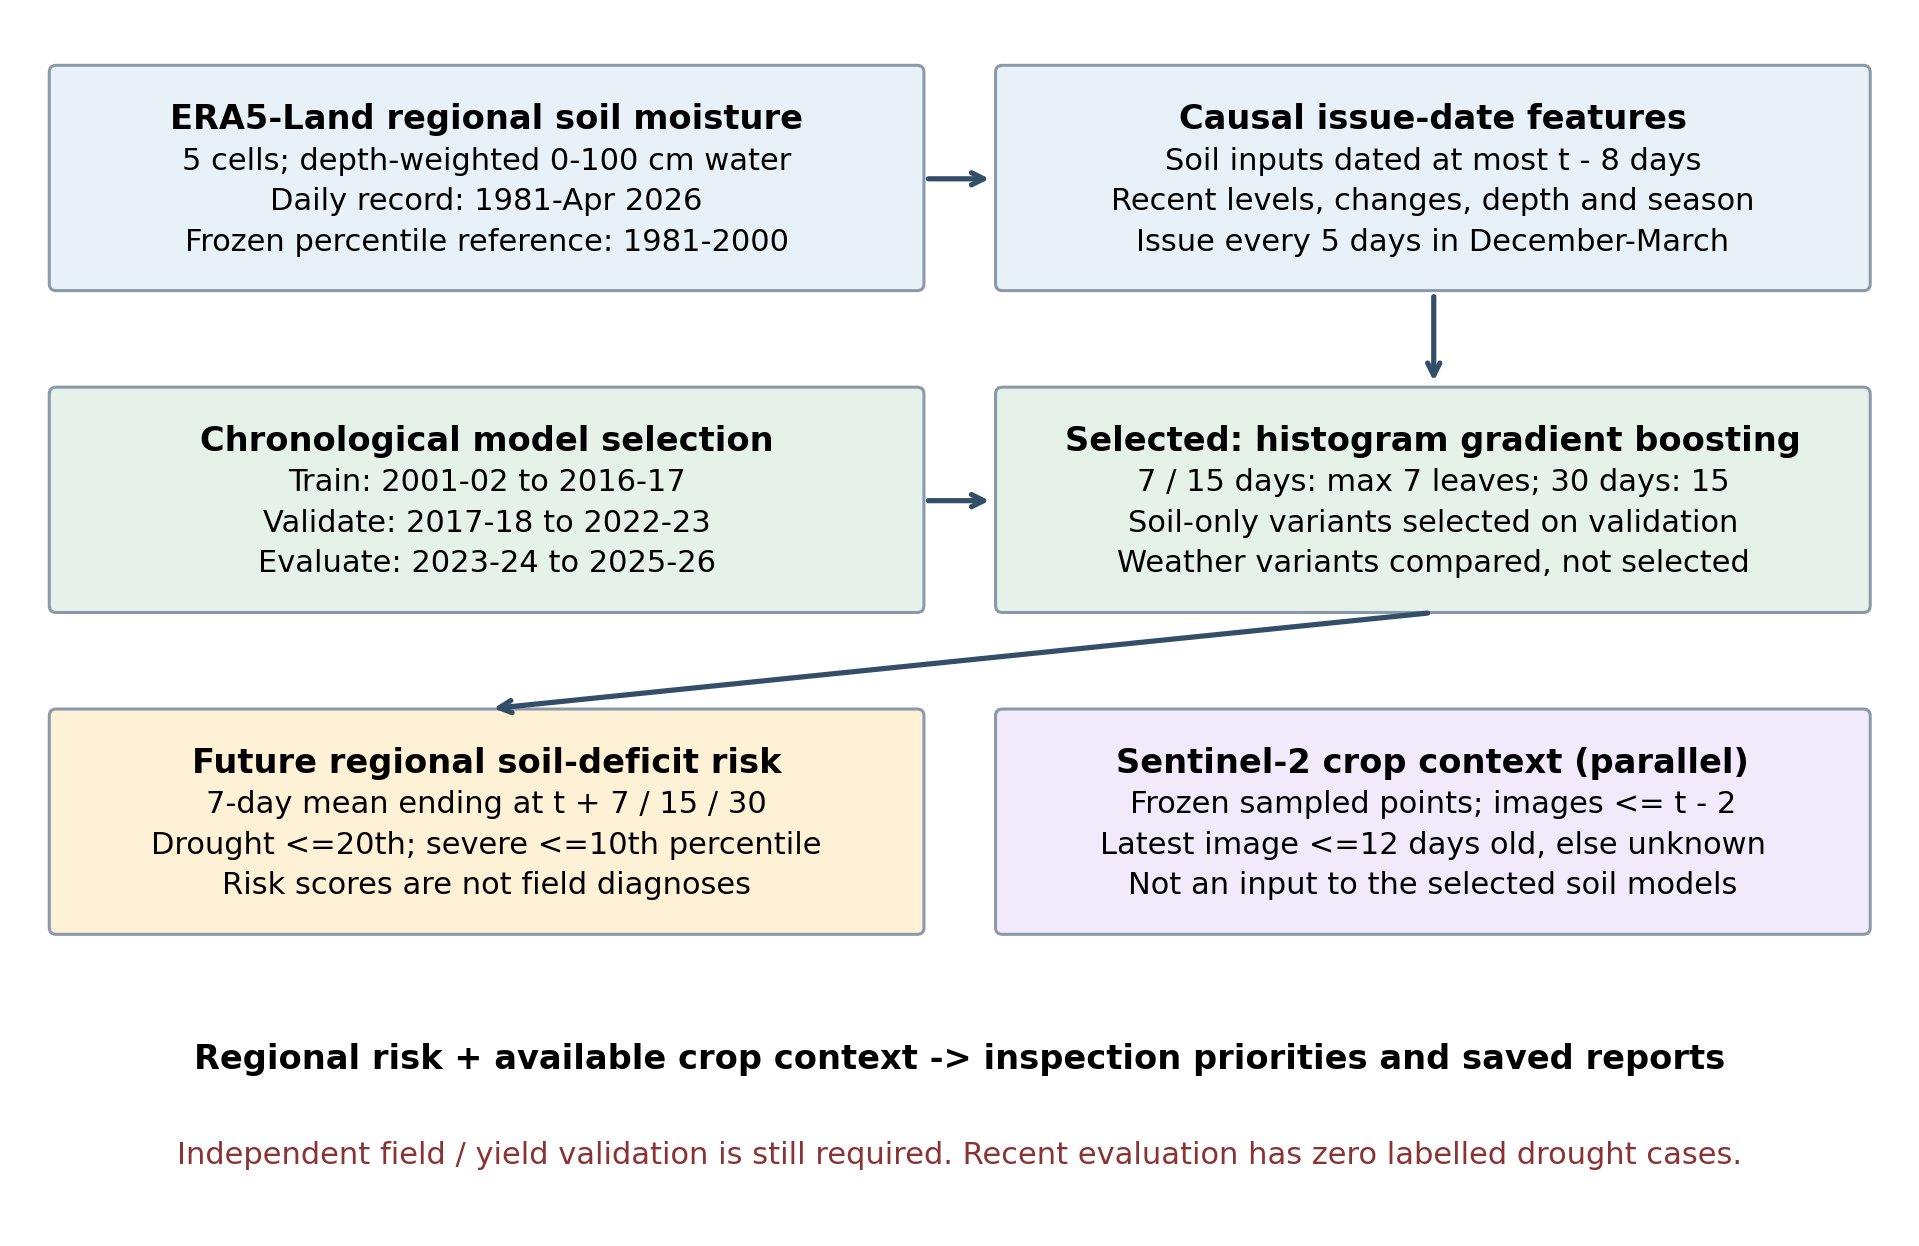
\includegraphics[width=0.95\textwidth]{figures/fig9_rabi_soil_drought_architecture.png}
\caption{Final rabi drought workflow. Satellite imagery supplies parallel crop context; it is not a feature in the selected regional soil-only models. The historical reference, supervised split and availability cutoffs are distinct.}
\label{fig:r_soil_arch}
\end{figure}\subsubsection{Primary evaluation: no positive drought targets}
\textbf{The 2023-24 to 2025-26 evaluation contains zero drought-labelled targets at every horizon.} The selected models issue zero warnings. Drought recall, average precision and ROC-AUC are therefore not estimable; a no-warning rule also succeeds on these rows. This evaluation cannot demonstrate drought-detection skill, and the reference was not changed to manufacture positive cases.
\begin{table}[H]
\centering\small
\caption{Primary historical evaluation of the soil model. Rows are correlated cell-issue forecasts, not independent drought episodes.}
\label{tab:r_soil_primary}
\begin{tabularx}{\textwidth}{@{}lXrrrl@{}}
\toprule
Horizon & Selected model & Rows & Dry targets & Warnings & Recall / AUC \\
\midrule
7 & HGB leaves7 soil & 375 & 0 & 0 & Not estimable \\
15 & HGB leaves7 soil & 375 & 0 & 0 & Not estimable \\
30 & HGB leaves15 soil & 375 & 0 & 0 & Not estimable \\
\bottomrule
\end{tabularx}
\end{table}\subsubsection{Earlier diagnostic backtest: continuation versus new onset}
An additional backtest trains on 2001-02 to 2013-14, validates on 2014-15 to 2016-17, and evaluates 2017-18 to 2019-20. It was chosen after inspecting drought prevalence and is \textbf{post hoc diagnostic evidence}, not an untouched confirmatory test. Its models and thresholds are selected independently on the earlier validation period and differ from the main selections. All positive evaluation targets occur in the 2018-19 season.
\begin{table}[H]
\centering\small
\caption{Earlier diagnostic backtest, all issue dates (including ongoing drought). Precision and recall describe repeated cell-dates.}
\label{tab:r_soil_back}
\begin{tabularx}{\textwidth}{@{}lXrrrr@{}}
\toprule
Horizon & Earlier selected model & Caught / dry & Warnings & Precision & Recall \\
\midrule
7 & Logistic soil & 26 / 35 & 45 & 57.8\,\% & 74.3\,\% \\
15 & HGB leaves7 soil+weather & 25 / 30 & 49 & 51.0\,\% & 83.3\,\% \\
30 & HGB leaves7 soil & 15 / 29 & 69 & 21.7\,\% & 51.7\,\% \\
\bottomrule
\end{tabularx}
\end{table}The new-onset subset retains only rows whose true issue-day soil indicator is above the 20th percentile. That issue-day truth is used only for retrospective scoring; predictor inputs still stop at $t-8$. There are 337 eligible rows, with only 6, 8 and 15 positive targets at 7, 15 and 30 days. At 15 days, the learned model catches \textbf{3 of 8} positives with 21.4\,\% precision; conditional transition catches \textbf{6 of 8} with 35.3\,\% precision. Thus the selected learned model has not shown an advantage over this simple baseline for new onset.
\begin{figure}[H]\centering
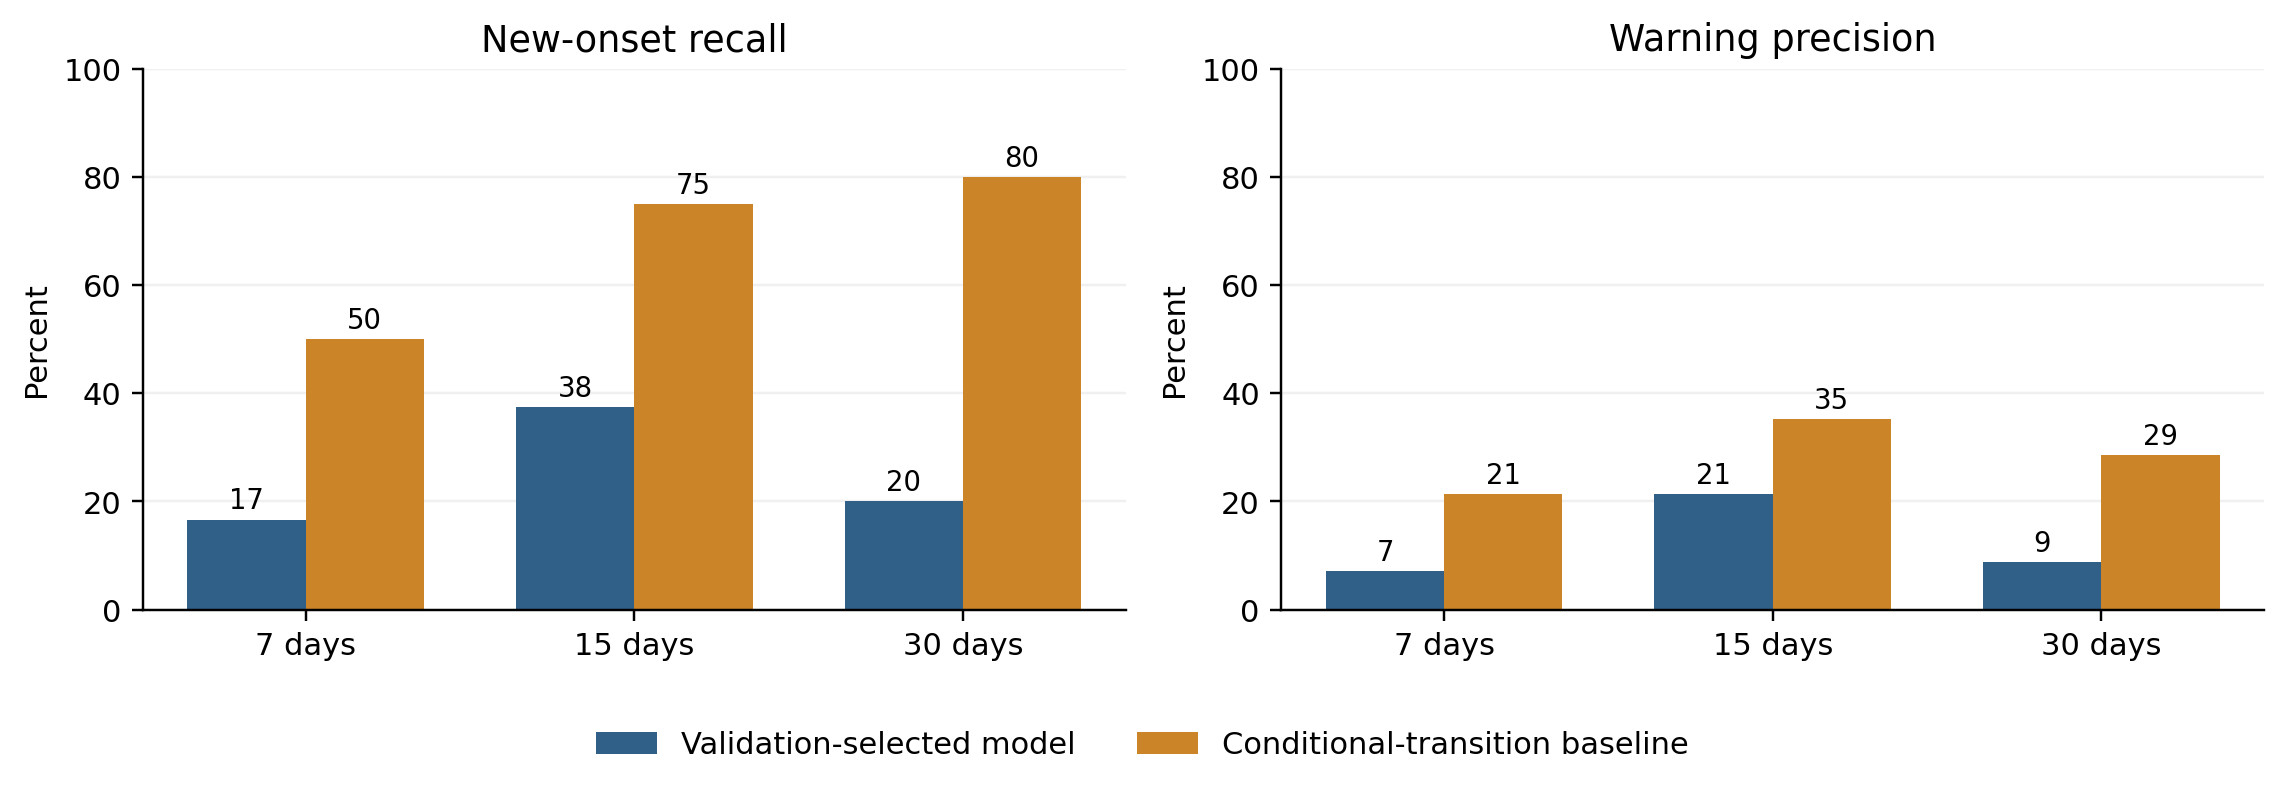
\includegraphics[width=0.95\textwidth]{figures/res_r_soil_new_onset.png}
\caption{Post hoc 2017-18 to 2019-20 new-onset comparison. Models were selected on earlier validation data, not these scores. Small, correlated cell-date counts preclude a claim of reliable independent-event performance.}
\label{fig:r_soil_onset}
\end{figure}\subsubsection{Dependence on the soil-moisture product}
A separate sensitivity check computes the same reference-period percentile definition using NASA POWER MERRA-2 root-zone wetness (a coarser, rounded product). On the 15-day target dates, ERA5-Land labels no drought cases in the three recent seasons, whereas MERRA-2 labels 15, 2 and 0 of 125 cell-dates respectively. Neither product is field truth. This disagreement limits conclusions about actual crop drought; it is not a reason to select whichever product agrees best with declarations.
\begin{figure}[H]\centering
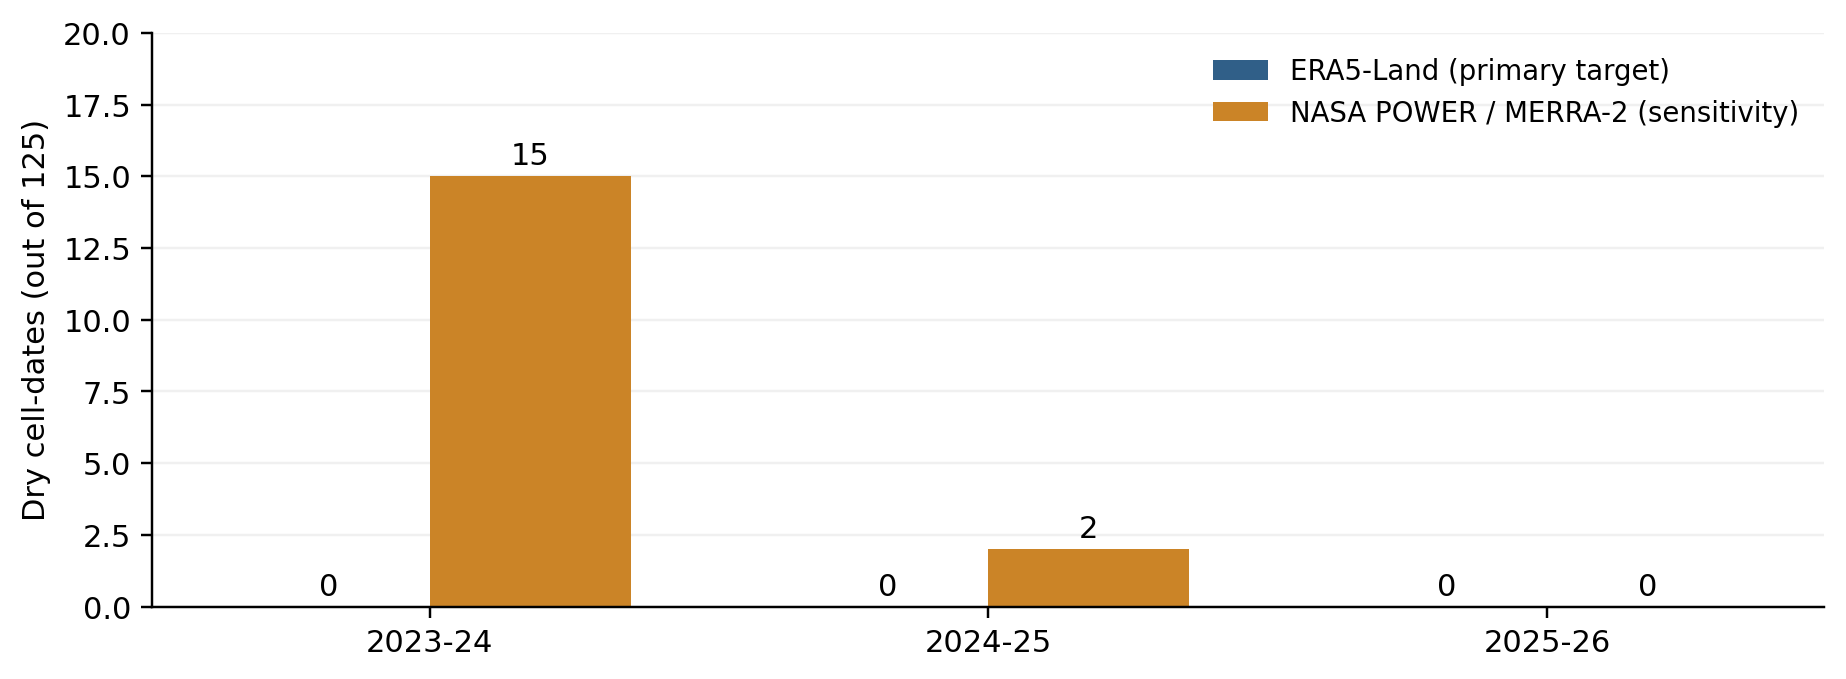
\includegraphics[width=0.85\textwidth]{figures/res_r_soil_product_sensitivity.png}
\caption{Soil-product sensitivity on 15-day target dates. Counts are regional cell-dates, not fields, mandals or independent drought episodes; each season has 125 target rows.}
\label{fig:r_soil_products}
\end{figure}\subsubsection{Operational output and present status}
The runnable workflow saves dated regional 7/15/30-day scores, source dates, input snapshots, provenance hashes, point-level crop context, inspection priorities, GeoJSON and an HTML report. Satellite context requires an image dated at most $t-2$ and no more than 12 days old; missing imagery is \emph{unknown}, not no crop. A 1 March 2026 replay reproduced all 15 saved research predictions and had recent imagery for 1,349 of 1,350 sampled points. The 23 November 2026 run is outside the December--March issue season and correctly produces no seasonal forecasts; current satellite context awaits a fresh export.

The software tests and artifact audit check implementation and reproducibility, not agricultural validity. Independent field-observation templates are supplied but contain no verified field outcomes. \textbf{The software is operational; reliable new agricultural-drought prediction is not yet demonstrated.} The immediate scientific priority is independent water-stress or yield evidence, more drought-bearing seasons/regions, and comparison with conditional transition on the same new-onset population. Future evaluation must preserve missing-data coverage and the distinction between regional water deficit and field crop damage.
